
\chapter{Curses, Blessings, and Surprises in High Dimensions}
\label{c:surprises}


Most of the material in this book will naturally ``live'' in the context of high dimensions, either motivated by the analysis of high dimensional data or by associating with networks a space whose dimension is the number of network nodes, %or by taking advantage of the celebrated phenomenon of concentration of measure,
to name a few. This chapter is about High Dimensions. It discusses the curse of dimensionality, but also many of its blessings. The first is caused by the exponential increase in volume associated with adding extra dimensions to Euclidean space. The latter is a manifestation of an intriguing phenomenon called the concentration of measure. This concentration phenomenon will give rise to many surprising facts about high dimensional geometry that we will discuss.
Since several of the results discussed in this chapter require basic tools from probability, we will also review some fundamental probabilistic concepts.

\subsubsection{The curse of dimensionality}

The {\em curse of dimensionality} refers to the fact that many algorithmic approaches to problems in
$\R^d$ become {\em exponentially} more difficult as the dimension $d$ grows. The expression ``curse of dimensionality'' was coined by Richard Bellman to describe the problem caused by the exponential increase in volume associated with adding extra dimensions to Euclidean space~\cite{bellman1957}.



For instance, if we want to sample the unit interval such that the distance between adjacent points is at most 0.01,
then 100 evenly-spaced sample points suffice; an equivalent sampling of a five-dimensional unit hypercube with a grid with a spacing of 0.01 between adjacent points would require $10^{10}$ sample points. Thus, a modest increase in dimensions results in a dramatic increase in required data points to cover the space at the same density.



Intimately connected to the curse of dimensionality is the problem of {\em overfitting} and {\em underfitting}. Here, overfitting refers to the issue that an algorithm may show good performance on the training data, but poor generalization to other data. Underfitting in turn, corresponds to poor performance on the training data (and poor generalization to other data). This problem manifests itself in many machine learning algorithms.

We will discuss a toy example from image classification in more detail to illustrate the underlying issues.
Assume we want to classify images into two groups, cars and bicycles, say. From the vast number of images depicting cars or bicycles, we are only able to obtain a small number of training images, say five images of cars and five images of bicycles. We want to train a simple linear classifier based on these ten labeled training images to correctly classify the remaining unlabeled car/bicycle images. We start with a simple feature, e.g.\ the amount of red pixels in each image.
However, this is unlikely to give a linear separation of the training data. We add more features and eventually the training images become linearly separable. This might suggest that increasing the number of features until perfect classification of the training data is achieved, is a sound strategy. However, as we {\em linearly increase} the dimension of the feature space, the density of our training data {\em decreases exponentially} with the feature dimension.

In other words, to maintain a comparable density of our training data, we would need to increase the size of the dataset exponentially -- the curse of dimensionality.
Thus, we risk producing a model that could be very good at predicting the target class on the training set, but it may fail miserably when faced with new data.  This means that our model does not {\em generalize} from the training data to the test data, leading to large {\em generalization error}.  The generalization error is an important concept in data science and machine learning, since it measures how accurately an algorithm can predict outcomes for new, unseen data.  As such, it indicates the data science model's ability to perform well beyond the training data, and is closely related to the concept of overfitting.


%\section{Surprises in High Dimensions}
\section{Geometry of spheres and cubes in high dimension}

When we peel an orange, then after having removed the rind we are still left with the majority of the orange. Suppose now we peel a $d$-dimensional orange for large $d$, then after removing the orange peel we would be left with essentially nothing.
The reason for this -- from a healthy nutrition viewpoint discouraging -- fact is that for a $d$-dimensional unit ball almost all of its volume is concentrated near the boundary sphere. This is just one of many surprising phenomena in high dimensions. Many of these surprises are actually a manifestation of some form of concentration of measure that we will analyze in more detail in the next section (and then these surprises are no longer so startling).


When introducing data analysis concepts, we typically use only a few dimensions in order to facilitate visualization.
However, our intuition about space, which is naturally based on two and three dimensions, can often be misleading in high dimensions.
Many properties of even very basic objects become counterintuitive in higher dimensions. Understanding these paradoxical properties is essential
in data analysis as it allows us to avoid pitfalls in the design of algorithms and statistical methods for high-dimensional data.
It is therefore instructive to analyze the shape and properties of some basic geometric forms that we understand very well
in dimensions two and three, in high dimensions.

To that end, we will look at some of the
properties of the sphere and the cube as the dimension increases.
The $d$-dimensional hyperball of radius $R$ is defined by
$$B^d(R) =\{x \in \R^d : x_1^2 + \dots +x_d^2 \le R^2\},$$ the $d$-dimensional hypersphere (or $d$-sphere) of radius $R$ is given by
$$S^{d-1}(R) =\{x \in \R^d : x_1^2 + \dots +x_d^2 = R^2\},$$
and the $d$-dimensional hypercube with side length $2R$  is the subset of $\R^d$ defined as the $d$-fold product of
intervals $[-R, R]$:
$$C^d(R) = \underbrace{ [-R,R] \times  \dots  \times [-R,R]}_{\text{$d$ times}}.$$
If there is no danger of confusion, we may write $B^d$ for the unit ball $B^d(1)$, $S^{d-1}$ for the unit sphere $S^{d-1}(1)$, and
$C^d$ for the unit hypercube $C^d(\frac{1}{2})$.



\subsection{High dimensional geometry and high dimensional probability} 

In the rest of this section we will establish a variety of (at first) surprising properties of high dimensional geometry. To illustrate the connections between geometry and probability we will derive some of the results first using analytical tools (computing volumes and integrals) and then using tools from Probability, namely concentration inequalities (which the reader might agree gives more elegant arguments). The goal here is not to get the best bounds, but to illustrate these properties and showcase the duality between geometry and probability.

%\subsection{Geometry of Spheres and Balls in High Dimension}
\subsubsection{Volume of the hyperball}

\begin{proposition}
The volume of $B^d(R)$ is given by
\begin{equation}
\label{volsphere}
\Vol(B^d(R)) = \frac{\pi^{\frac{d}{2}} R^d}{\frac{d}{2}\ \Gamma(\frac{d}{2})}.
\end{equation}
\end{proposition}

\begin{proof}
The volume of $B^{d}(R)$ is given by
\begin{equation}\label{volume_dsphere}
\Vol(B^d(R)) = \int_0^R s_d r^{d-1} dr =  \frac{s_d R^d}{d},
\end{equation}
where $s_d$ denotes the (hyper-)surface area of a unit $d$-sphere. A unit $d$-sphere must satisfy
$$s_d \int_0^{\infty} e^{-r^2} r^{d-1} dr = \underbrace{\int_{-\infty}^{\infty} \cdots \int_{-\infty}^{\infty}}_{\text{$d$ times}} e^{-(x_1^2 + \cdots +x_d^2)}  dx_1 \cdots d x_d = \Big( \int_{-\infty}^{\infty} e^{-x^2} dx \Big)^d.$$
Recall that the Gamma function is given by
$$\Gamma(n) = \int_0^\infty r^{n-1} e^{-r}  dr = 2 \int_0^\infty e^{-r^2} r^{2n-1} dr,$$
hence
$\frac{1}{2} s_d \Gamma(\frac{d}{2}) = \Big[ \Gamma(\frac{1}{2}) \Big]^d = \big( \pi^{\frac{1}{2}}\big)^d,$
and thus
$s_d = \frac{2 \pi^{\frac{d}{2}} }{\Gamma(\frac{d}{2})}.$
Plugging this expression into~\eqref{volume_dsphere} gives
\begin{equation}
\label{volsphere}
\Vol(B^d(R)) = \frac{\pi^{\frac{d}{2}} R^d}{\frac{d}{2}\ \Gamma(\frac{d}{2})}.
\end{equation}
%
\end{proof}

Recall that for even $d$, we have $\Gamma(d/2) = (d/2 - 1)!$. To understand the asymptotic behavior $\Vol(B^d(R))$ we can use the celebrated Stirling's Formula,
\begin{align*}
  \Gamma(n) \approx \sqrt{\frac{2\pi}{n}}\left(\frac{n}{e}\right)^n
\end{align*}
we obtain an approximation for the volume of the unit $d$-ball for large $d$
\begin{align}\label{approxvolume}
  \Vol(B^d) \approx \frac{1}{\sqrt{d\pi}} \Big( \frac{2\pi e}{d} \Big)^{\frac{d}{2}},
\end{align}
where $\approx$ means that the quotient goes to $1$ as the relevant parameter, in this case $d$, goes to $\infty$.

Since the denominator in the parenthesis of equation~\eqref{approxvolume} goes to infinity,
the volume of the unit $d$-sphere goes rapidly to $0$ as the dimension $d$ increases to infinity, see also Figure~\ref{fig:volume_sphere}. Notice that this would still be the case for any fixed radius $R$.

Thus, unit spheres in high dimensions have almost no volume---compare this to the unit cube, which has volume $1$ in any dimension. For $B^d(R)$ to have volume equal to 1, its radius $R$ must be
approximately (asymptotically) equal to $\sqrt{\frac{d}{2\pi e}}$.


\begin{figure}
\centering

\includegraphics[width=0.8\textwidth]{figures/Chapter2-volume_sphere}
\caption{The volume of the unit $d$-ball using the exact formula in equation~\eqref{volsphere}. The volume reaches its maximum for $d=5$ and decreases rapidly to zero with increasing dimension $d$.}
\label{fig:volume_sphere}
\end{figure}

\subsubsection{Concentration of the volume of a ball near its equator}


If we take an orange and cut it into slices, then the slices near the center are larger since the sphere is wider there. This effect increases dramatically (exponentially with the dimension) with increasing dimension.
Assume we want to cut off a slab around the ``equator\footnote{To define the ``equator'' of a the $d$-dimensional ball, we need to pick a ``north pole'' as reference. Without loss of generality we could pick the unit vector in the $x_1$-direction as defining ``north''.}'' of the $d$-unit ball such that 99\% of its volume is contained inside the slab. In two dimensions the width of the slab has to be almost 2, so that 99\% of the volume are captured by the slab. But as the dimension increases the width of the slab gets rapidly smaller. Indeed, in high dimensions only a very thin slab is required, since nearly all the volume of the unit ball lies a very small distance away from the equator.  The following theorem makes the considerations above precise.


%\begin{theorem}
%Almost all the volume of $B^d(R)$ lies near its equator. To be more precise, given any fixed (positive) latitude, let $P$ be the subset of the ball above that latitude (the ball cap of points whose first coordinate is above a positive value $p_0$). Then, for large enough $d$,
%\[                                                 
%\frac{2 \Vol(P)}{\Vol(B^{d})}  \le e^{-\frac{d-1}{2}p_0^2}.
%\]
%%  the volume of the ball further from the  that latitude
%%The $d-1$-dimensional volume of the slice at $x$ of a $d$-ball of total
%%volume 1 approaches the value $e^{1/2} e^{-\pi e x^2}$ as $d \to \infty$.
%\end{theorem}

\begin{fact}\label{fact:spheremostlyinequator}
Almost all the volume of $B^d(R)$ lies near its equator.
%  the volume of the ball further from the  that latitude 
%The $d-1$-dimensional volume of the slice at $x$ of a $d$-ball of total
%volume 1 approaches the value $e^{1/2} e^{-\pi e x^2}$ as $d \to \infty$.
\end{fact}


\begin{proof}
It suffices to prove the result for the unit $d$-ball.
Without loss of generality we pick as ``north'' the direction $x_1$. The intersection of the sphere with the plane $x_1=0$  forms our equator, which is formally given by the $d-1$-dimensional region
$\{x: \|x\| \le 1, x_1=0\}$, where $\|x\|$ is the Euclidean norm\footnote{Throughout the book,  $\|\cdot \|$ denotes the Euclidean norm if we are dealing with vectors and it denotes the operator norm if we are dealing with matrices or operators.} of $x$. This intersection is a sphere of dimension $d-1$ with volume $\Vol(B^{d-1})$ given by
the $(d-1)$-analog of formula~\eqref{volsphere} with $R=1$.

We now compute the volume of $B^d$ that lies between $x_1=0$ and $x_1=p_0$.
Let $P_0=\{x: \|x\|\le 1, x_1\ge p_0\}$ be the ``polar cap'', i.e., part of the sphere above the slab of width $2p_0$ around the equator.
To compute the volume of the cap $P$ we will integrate over all slices of the cap from $p_0$ to 1.  
Each such slice will be a sphere of dimension $d-1$ and radius $\sqrt{1-p^2}$, hence its  volume is
$(1-p^2)^{\frac{d-1}{2}} \Vol(B^{d-1})$. Therefore
$$\Vol(P) = \int_{p_0}^1 (1-p^2)^{\frac{d-1}{2}} \Vol(B^{d-1}) \, dp = \Vol(B^{d-1})   \int_{p_0}^1 (1-p^2)^{\frac{d-1}{2}} \, dp.$$
Using $e^x \ge 1+x$ for all $x$ we can upper bound  this integral by
\begin{eqnarray*}
\Vol(P) &\le& \Vol(B^{d-1}) \int_{p_0}^\infty e^{-\frac{d-1}{2}p^2} \, dp = \Vol(B^{d-1})\sqrt{\frac{2}{d-1}} \int_{p_0 \sqrt{\frac{d-1}{2}}}^{\infty} e^{-u^2}\,du \\
&=& \Vol(B^{d-1}) \sqrt{\frac{\pi}{2(d-1)}}\erfc\left(p_0 \sqrt{\frac{d-1}{2}} \right),
\end{eqnarray*}
where $\erfc(x) = \frac{2}{\sqrt{\pi}}\int_x^{\infty} e^{-u^2}\,du$ is the complementary error function. The upper bound $\erfc(x) \leq \frac{e^{-x^2}}{\sqrt{\pi} x}$ gives
\begin{equation}\label{eq:chapter2:volBvolP:1}
\Vol(P) \le \Vol(B^{d-1}) \sqrt{\frac{\pi}{2(d-1)}}\frac{e^{- \frac{d-1}{2}p_0^2}}{\sqrt{\pi} p_0 \sqrt{\frac{d-1}{2}}} =  \frac{\Vol(B^{d-1})}{d-1}\frac{e^{- \frac{d-1}{2}p_0^2}}{ p_0}
\end{equation}




Recall, from~\eqref{volsphere} that $\Vol(B^{d}) = \frac{\pi^{\frac{d}{2}} }{\frac{d}{2}\ \Gamma(\frac{d}{2})}$, so, for $d$ large enough (since $\frac{\Gamma(\frac{d}{2})}{\Gamma(\frac{d-1}{2})} \approx \sqrt{\frac{d}2}$),
\begin{equation}\label{eq:chapter2:volBvolP:2}
\Vol(B^{d-1}) = \frac{\pi^{-1/2}}{\frac{d-1}{d}} \frac{\Gamma(\frac{d}{2})}{\Gamma(\frac{d-1}{2})}\Vol(B^{d}) \leq \frac{d-1}2\Vol(B^{d}).
\end{equation}
Finally, combining~\eqref{eq:chapter2:volBvolP:1} and~\eqref{eq:chapter2:volBvolP:2} shows that the ratio between the volume of the polar caps and the entire hypersphere is bounded by
$$\frac{2 \Vol(P)}{\Vol(B^{d})} \le (d-1)\frac{ \Vol(P)}{\Vol(B^{d-1})} \le \frac{1}{p_0}\exp\left(-\frac{d-1}{2}p_0^2\right).$$
The expression above shows that this ratio decreases exponentially as both $d$ and $p$
increase, proving our claim that the volume of the sphere concentrates strongly around its equator.

\end{proof}

%A consequence of the considerations above is that picking a point at random on the unit $d$-sphere is
%quite similar to picking a point

\subsection{Concentration of the volume of a ball on shells}

We consider two concentric balls $B^d(1)$ and $B^d(1-\eps)$. Using equation~\eqref{volsphere}, the ratio of their volumes is
\begin{align}
\frac{\Vol\big(B^d(1-\eps)\big)}{\Vol\big(B^d(1)\big)} = (1-\eps)^d.
\end{align}
Clearly, for every $\eps$ this ratio tends to zero as $d \to \infty$. This implies that the spherical shell given by the region between $B^d(1)$ and $B^d(1-\eps)$ will contain most of the volume of $B^d(1)$  for large enough $d$ even if $\eps$ is very small. How quickly does the volume concentrate at the surface of $B^d(1)$? We choose $\eps$ as a function of $d$, e.g. $\eps = \frac{t}{d}$, then
\[
\frac{\Vol(B^d(1-\eps))}{\Vol(B^d(1))} = \Big(1-\frac{t}{d}\Big)^d \to e^{-t}.
\]
Thus, almost all the volume of $B^d(R)$ is contained in an annulus of width $R/d$.

Therefore, if we peel a $d$-dimensional orange---and even if we peel it very carefully so that we remove only a very thin layer of its peel---we will have removed most of the orange and are left with almost nothing.





\subsubsection{Geometry of the hypercube} \label{ss:hypercube}

We have seen that most of the volume of the hypersphere is concentrated near its surface. A similar result also holds for the hypercube, and it is indeed a tendency for high-dimensional geometric objects. Yet, the hypercube exhibits
an even more interesting volume concentration behavior, which we will establish below.

We start with a basic observation.
%\begin{proposition}
%Let $n \to \infty$, then $\Vol(C^d(s)) \to \infty$  if $s > \frac{1}{2}$,  $\Vol(C^d(s)) \to 0$ if $s < \frac{1}{2}$
%and $\Vol(C^d(s)) =1$ if $s = \frac{1}{2}$.
%\end{proposition}
\begin{proposition}
The hypercube $C^d$ has volume 1 and diameter $\sqrt{d}$.
\end{proposition}
The above proposition, although mathematically  trivial, hints already at a somewhat counterintuitive behavior of the cube in high dimensions. Its corners seem to get ``stretched out'' more and more, while the rest of the cube must ``shrink'' to keep the volume constant. This property becomes even more striking when we compare the cube with the sphere as the dimension increases.

\begin{figure}[ht!]
  \centering
  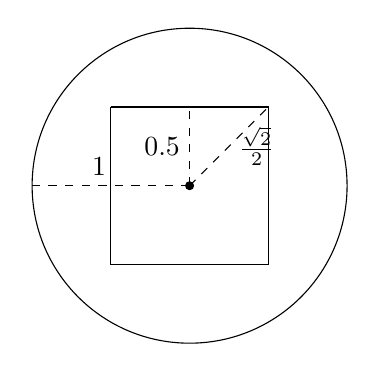
\begin{tikzpicture}[scale=0.2]
  \draw (-5,5) -- (5,5) -- (5,-5) -- (-5,-5) -- (-5,5);
  \node[draw,circle,fill,scale=0.3] (origin) at (0,0) {};
  \draw[dashed] (0,0) -- node [left,midway] (half) { 0.5} (0,5);
  \draw[dashed] (0,0) -- node [right,midway] (root) {$\frac{\sqrt{2}}{2}$} (5,5);
  \draw[dashed] (0,0) -- node [above,near end] (one) {\qquad 1} (-10,0);
  \draw (0,0) circle (10);
  \end{tikzpicture}
  \caption{$2$-dimensional unit sphere and unit cube, centered at the origin.}
  \label{2dim}
\end{figure}

In two dimensions (Figure~\ref{2dim}), the unit square is completely contained in the unit sphere.  The distance from the center to a vertex (radius of the circumscribed sphere) is $\frac{\sqrt{2}}{2}$ and the apothem (radius of the inscribed sphere) is $\frac{1}{2}$.  In four dimensions (Figure~\ref{4dim}), the distance from the center to a vertex is $1$, so the vertices of the cube touch the surface of the sphere.  However, the apothem is still $\frac{1}{2}$.  The result, when projected in two dimensions no longer appears convex, however all hypercubes are convex.  This is part of the strangeness of higher dimensions - hypercubes are both convex and ``pointy.''  In dimensions greater than $4$ the distance from the center to a vertex is $\frac{\sqrt{d}}{2} > 1$, and thus the vertices of the hypercube extend far outside the sphere, cf.~Figure~\ref{ddim}.


\begin{figure}[ht!]
  \centering
  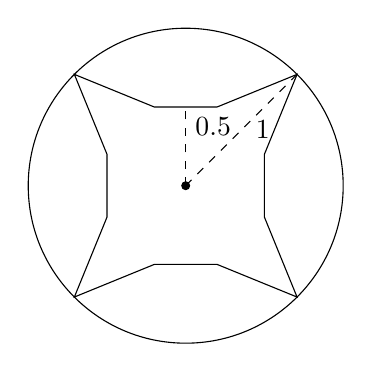
\begin{tikzpicture}[scale=0.2]
  \draw (2,5) -- (7.07,7.07) -- (5,2) -- ( 5,-2) -- (7.07,-7.07) -- (2,-5) -- (-2,-5) -- (-7.07,-7.07) -- (-5,-2) -- (-5,2) -- (-7.07,7.07) -- (-2,5) -- (2,5);
  \node[draw,circle,fill,scale=0.3] (origin) at (0,0) {};
  \draw[dashed] (0,0) -- node [right,near end] (half) {0.5} (0,5);
  \draw[dashed] (0,0) -- node [right,midway] (one) {\,1} (7.07,7.07);
  \draw (0,0) circle (10);
  \end{tikzpicture}
  \caption{Projections of the $4$-dimensional unit sphere and unit cube, centered at the origin (4 of the 16 vertices of the hypercube are shown).}
  \label{4dim}
\end{figure}

\begin{figure}[ht!]
  \centering
  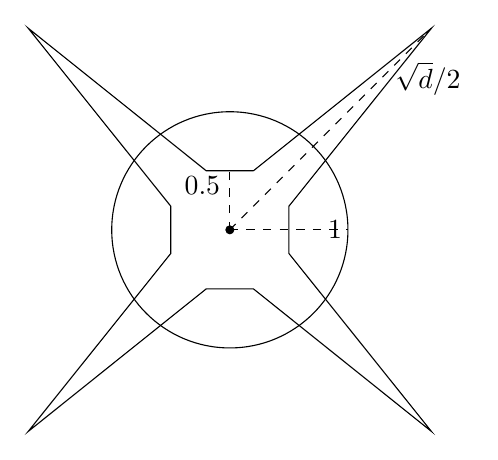
\begin{tikzpicture}[scale=0.15]
  \draw (2,5) -- (17.07,17.07) -- (5,2) -- ( 5,-2) -- (17.07,-17.07) -- (2,-5) -- (-2,-5) -- (-17.07,-17.07) -- (-5,-2) -- (-5,2) -- (-17.07,17.07) -- (-2,5) -- (2,5);
  \node[draw,circle,fill,scale=0.3] (origin) at (0,0) {};
  \draw[dashed] (0,0) -- node [left,near end] (half) {0.5} (0,5);
    \draw[dashed] (0,0) -- node [right,near end] (half) {1} (10,0);

  \draw[dashed] (0,0) -- node [right,near end] (one) {\,$\sqrt{d}/2$} (17.07,17.07);
  \draw (0,0) circle (10);
  \end{tikzpicture}
  \caption{Projections of the $d$-dimensional unit sphere and unit cube, centered at the origin (4 of the $2^d$ vertices of the hypercube are shown).}
  \label{ddim}
\end{figure}

The considerations above suggest the following observation:
%\smallskip

%\centerline{
%{\em ``Most of the volume of the high-dimensional cube is located in its corners.''}}



\begin{fact}\label{fact:hypercubemostlycorners}
Most of the volume of the high-dimensional cube is located in its corners.
\end{fact}

%\smallskip

\begin{proof}
Let $C^d$ denote the unit hypercube. The subset $Q_R$ of $C^d$ of points $x\in\RR^d$ whose distance to the center is smaller that $R$ ($Q_R = \{x\in C^d: \|x\|\leq R\}$) is given by $Q = C^d\cap B^d(R)$. Thus
\[
\frac{\vol(Q_R)}{\vol(C^d)} = \vol(Q) \le B^d(R) \approx \frac{1}{\sqrt{d\pi}} \Big( \frac{2\pi e R^2}{d} \Big)^{\frac{d}{2}},
\]
which goes to zero as long as $R<\sqrt{\frac{d}{2\pi e}}$. This shows that most of the volume of $C^d$ lies in points at distance of order $\sqrt{d}$ of the center.

\end{proof}




\section{Basic concepts from probability}

We briefly review some fundamental concepts from probability theory, which are helpful or necessary to understand the blessings of dimensionality and some of the surprises encountered in high dimensions. More advanced probabilistic concepts
will be presented in Chapter~\ref{c:probability-gaussiananalysis}.
We assume that the reader is familiar with elementary probability as is covered in introductory probability courses (see, for example~\cite{durrett2019probability,ross2014introduction}).

The two most basic concepts in probability associated with a random variable $X$ are {\em expectation} (or {\em mean}) and {\em variance}, denoted by
$$\E[X] \qquad \text{and} \qquad \Var(X) := \E [ (X- \E [X])^2 ],$$
respectively. 

A useful identity is the {\em Law of Total Variance}. This fundamental theorem in probability theory decomposes the variance of a random variable into two distinct components: the variance that can be explained by another variable and the variance that remains as ``noise.'' Let $X$ and $Y$ be random variables on the same probability space, and assume that the variance of $X$ is finite. The Law of Total Variance states
\begin{eqnarray}\label{eq:totalvariance}
\Var(X) = \E[\Var(X \mid Y)] + \Var(\E[X \mid Y]).\end{eqnarray}
The two terms have a natural interpretation:
\begin{itemize}
\item $\E[\Var(X \mid Y)]$ is the unexplained variance --- the variability in $X$ that
persists even after knowing $Y$.
\item
$\Var(\E[X \mid Y])$ is the is the variance of the conditional mean --- the variability in $X$ explained by $Y$. 
\end{itemize}




An important tool to describe probability distributions is the {\em moment generating function} (MGF) of $X$, defined by
\begin{equation}\label{eq:MomentGeneratingFunction}    
M_X(t) = \E [e^{tX}], \quad t\in \R,
\end{equation}
the choice of nomenclature can be easily justified by expanding $M_X(t)$ in a series.
The $p$-th moment of $X$ is defined by $\E[X^p]$ for $p >0$ and the $p$-th absolute moment is $\E[|X|^p]$.

We can introduce $L^p$-norms of random variables by taking the $p$-th root of moments, i.e.,
$$\|X\|_{L^p} := \big(\E[|X|^p]\big)^{\frac{1}{p}}, \qquad p \in [0,\infty],$$
with the usual extension to $p=\infty$ by setting
$$\|X\|_{\infty} := \ess \sup |X|.$$

Let $(\Omega,\Sigma,\P)$ be a probability space, where $\Sigma$ denotes a $\sigma$-algebra on the sample space
$\Omega$ and $\P$ is a probability measure on $(\Omega,\Sigma).$ For fixed $p$ the vector space
$L^p(\Omega,\Sigma,\P)$ consists of all random variables $X$ on $\Omega$ with finite $L^p$-norm, i.e.,
$$L^p(\Omega,\Sigma,\P) = \{X : \|X\|_{L^p} < \infty\}.$$
The random variable can be viewed as a (measurable) map $X:\Omega\to\RR$ (or $\CC$). We will usually not mention the underlying probability space. For example, we will often simply write $L^p$ for $L^p(\Omega,\Sigma,\P)$.

The case $p=2$ deserves special attention since $L^2$ is a Hilbert space with inner product and norm
$$\langle X, Y \rangle_{L^2} = \E[XY], \qquad \|X\|_{L^2} = \big(\E [X^2] \big)^{\frac{1}{2}},$$
respectively. Note that the {\em standard deviation} $\sigma(X):=\sqrt{\Var(X)}$ of $X$ can be written as
$$\sigma(X) = \| X - \E[X] \|_{L^2}.$$
The {\em covariance} of the random variables $X$ and $Y$ is
\begin{equation}
\label{covariance}
\cov(X,Y) = \E [ (X - \E[X]) (Y - \E [Y])]  = \langle X - \E[X], Y - \E [Y] \rangle_{L^2} .
\end{equation}


We recall a few classical inequalities for random variables. {\em H\"older's inequality} states that for random variables $X$ and $Y$ on a common probability space and $p,q \ge 1$ with $1/p +1/q =1$, there holds
\begin{equation}
\label{hoelder}
| \E [XY] | \le  \|X\|_{L^p} \|Y\|_{L^q}. %%(\E [|X|^p])^{1/p}  (\E [|Y|^q])^{1/q}.
\end{equation}
The special case $p=q=2$ is the {\em Cauchy-Schwarz inequality}
\begin{equation}
\label{cauchy-schwarz}
 | \E [XY] | \le \sqrt{ \E [|X|^2] \E [|Y|^2]}.
\end{equation}


{\em Jensen's inequality} states that for any random variable $X$ and a convex function $\phi: \R \to \R$, we have
\begin{equation}
\label{Jensen}
\phi(\E[X]) \le \E [\phi(X)].
\end{equation}

Since $\phi(x) = x^{q/p}$ is a convex function for $q\geq p \geq 0$, it follows immediately from Jensen's inequality that
$$\| X\|_{L^p} \le \|X\|_{L^q} \qquad \text{for $0 \le p \le q < \infty$.}$$

{\em Minkovskii's inequality} states that for any $p \in [0,\infty]$ and any random variables $X, Y$, we have
\begin{equation}
\label{minkovski}
\|X + Y\|_{L^p} \le  \|X \|_{L^p} + \|Y\|_{L^p},
\end{equation}
which can be viewed as the {\em triangle inequality}.


\bigskip

The {\em cumulative distribution function} of $X$ is defined by
$$F_X (t) =\P(X \le t), \quad t \in \R.$$
We have $\P\{X > t\} = 1 -F_X(t),$
where the function $t \mapsto \P \{ |X| \ge t \}$ is called the {\em tail} of $X$.
The following lemma establishes a close connection between expectation and tails.
\begin{proposition}[Integral identity]
\label{integralidentity}
Let $X$ be a non-negative random variable. Then
$$
\E[X] = \int_0^{\infty} \P \{X > t \} \, dt.$$
The two sides of this identity are either finite or infinite simultaneously.

\end{proposition}

Given an event $E$ with non-zero probability,$\P(\cdot |E)$ denotes conditional probability, furthermore for a random variable $X$ we use $\E[X|E]$ to denote the conditional expectation.

\subsection{Tail bounds}

{\em Markov's inequality} is a fundamental tool to bound the tail of a random variable in terms of its expectation.

\begin{proposition}\label{prop:markov}
For any non-negative real random variable $X$  we have
\begin{equation}
\label{markov}
\P \{ X \ge t \} \le \frac{ \E[X] }{ t } \qquad \text{for all $t  > 0$.}
\end{equation}
\end{proposition}

We provide two versions of the same proof, one using the language of conditional expectations.

\begin{proof}

Let ${\mathcal I}$ denote the event $\{X \ge t\}$. Then
$$\E[X] = \sum_{s  \in S} p(s) X(s) = \sum_{s \in {\mathcal I}} p(s) X(s) + \sum_{s \in {\mathcal I}^c} p(s) X(s),$$
where $p(s)$ denotes the probability of $s$; in case of continuous variables this should be replaced with the density function and $\sum$ with an integral.

Since $X$ is non-negative, it holds $\sum_{s \in {\mathcal I}^c} p(s) X(s) \ge 0$ and
$$\E[X] \ge \sum_{s \in {\mathcal I}} p(s) X(s) \ge t \sum_{s \in {\mathcal I}} p(s) = t \P\{{\mathcal I}\}.$$ 
\end{proof}

\begin{proof}[Using the language of conditional expectation]
$$\E[X] = \P(X<t) \E[X | X<t] + \P(X>t) \E[X | X\geq t], $$
where we take the product to be zero if the probability is zero.

Since $X$ is non-negative, it holds $ \P(X<t) \E[X | X<t] \geq 0$. Also,  $\E[X | X \geq t] > t$. Hence,
$$\E[X] \ge \P(X>t) \E[X | X>t] \ge t \P(X \geq t).$$

\end{proof}

An important consequence of Markov's inequality is  {\em Chebyshev's inequality}.
\begin{corollary}\label{chebyshev}
Let $X$ be a random variable with mean $\mu$ and variance $\sigma^2$. Then, for any $t>0$
\begin{equation}
\label{chebyshev}
\P \{ | X - \mu | \ge t \} \le \frac{ \sigma^2 }{ t^2}.
\end{equation}
\end{corollary}

Chebyshev's inequality, which follows by applying Markov's inequality to the non-negative random variable $Y = (X - \E[X])^2$, is a form of concentration inequality, as it guarantees that $X$ must be close to its mean $\mu$ whenever the variance of $X$ is small. Both, Markov's and Chebyshev's inequality are sharp, i.e., in general they cannot be improved.

Markov's inequality only requires the existence of the first moment. We can say a bit more if in addition the random variable $X$ has a moment generating function
in a neighborhood around zero, that is, there is a constant $b>0$ such that $\E [ e^{\lambda (X-\mu)}]$ exists for all $\lambda \in [0,b]$.
In this case we can apply Markov's inequality to the random variable $Y = e^{\lambda (X-\mu)}$ and obtain the generic {\em Chernoff bound}
\begin{equation}\label{basicchernoff}
\P \{ X -\mu \ge t \} = \P \{ e^{\lambda (X-\mu)} \ge e^{\lambda t} \} \le \frac{ \E[e^{\lambda (X-\mu)}] }{ e^{\lambda t} }.
\end{equation}
In particular, optimizing over $\lambda$ in order to obtain the tightest bound in~\eqref{basicchernoff} gives
$$
\log \P \{ X -\mu \ge t \} \le - \sup_{ \lambda \in [0,b]}  \{ \lambda t - \log \E[e^{\lambda (X-\mu)} ]  \}.
$$


\bigskip
{\em Gaussian random variables} are among the most important random variables.
A Gaussian random variable $X$ with mean $\mu$ and standard deviation $\sigma$ has a probability density function given by
\begin{equation} \label{def:gaussian}
\psi(t) = \frac{1}{\sqrt{2 \pi \sigma^2}} \exp\left( - \frac{(t-\mu)^2}{2\sigma^2}  \right).
\end{equation}
We write $X \sim {\mathcal N}(\mu,\sigma^2)$.
We call a Gaussian random variable $X$ with $\E[X] = 0$ and $\E[X^2] = 1$  a {\em standard Gaussian} or {\em standard normal}  (random
variable). In this case we have the following tail bound.


\begin{proposition}[Gaussian tail bounds] \label{prop:gaussian}
Let $X \sim {\mathcal N}(\mu,\sigma^2)$. Then for all $t>0$
\begin{equation}\label{gaussiantail}
 \P (X \ge \mu + t) \le e^{-t^2/2\sigma^2}.
\end{equation}
\end{proposition}


\begin{proof}
Without loss of generality we consider $\mu=0$ and $\sigma=1$, as it is straightforward to extend to the general case with a change of variables. We use the moment-generating function $\lambda \mapsto \E[e^{\lambda X}]$. A simple calculation gives
\begin{equation*}%\label{eq:gauss2}
\E[e^{\lambda X}] =   \frac{1}{\sqrt{2 \pi}} \int_{-\infty}^{\infty} e^{ \lambda x- x^2/2} \, dx =
\frac{1}{\sqrt{2 \pi}}   e^{  \lambda^2/2} \int_{-\infty}^{\infty} e^{ -(x- \lambda)^2/2} \, dx = e^{ \lambda^2/2},
\end{equation*}
where we have used the fact that $ \int_{-\infty}^{\infty} e^{ -(x- \lambda)^2/2} \, dx$  is just the entire Gaussian integral shifted and therefore its value is $\sqrt{2\pi}$.
%$\E[e^{\lambda X}] = e^{ \lambda^2/2}$.
We now apply  Chernoff's bound~\eqref{basicchernoff} and obtain $\P(X \geq t) \le \E[e^{\lambda X}]  e^{-\lambda t}$. Minimizing this expression over $\lambda$ gives $\lambda=t$ and thus $\P (X \geq t) \le e^{-t^2/2}$.
\end{proof}

\subsection{Sub-gaussian random variables}

\begin{definition}\label{def:subgaussian}
A random variable $X$ with mean $\mu = \E[X]$  is called {\em sub-Gaussian} if there is a positive number $\sigma$ such that
$$\E[e^{\lambda(X-\mu)}] \le e^{\sigma^2 \lambda^2/2}, \qquad \text{for all $\lambda \in \R$.}$$
\end{definition}
Note that $\sigma^2$ is not necessarily the variance of $X$. If $X$ satisfies the above definition, we also say that $X$ is sub-Gaussian with parameter $\sigma$, or $X$ is $(\mu,\sigma)$ sub-Gaussian in case we want to emphasize $\mu$ as well. Clearly, owing to the symmetry in the definition, $-X$ is sub-Gaussian if and only if $X$ is sub-Gaussian.
Obviously, any Gaussian random variable with variance $\sigma^2$ is sub-Gaussian with parameter $\sigma$.
We refer to~\cite{vershynin2018} for other, equivalent, definitions of sub-Gaussian random variables.

Combining the moment condition in Definition~\ref{def:subgaussian} with calculations similar to those that lead us to the Gaussian tail bounds in~\ref{prop:gaussian}, yields the following concentration inequality for sub-Gaussian random variables.
\begin{proposition}[Sub-Gaussian tail bounds] \label{prop:subgaussian}
Assume $X$ is sub-Gaussian with parameter $\sigma$. Then for all $t>0$
\begin{equation}\label{subgaussiantail}
 \P (|X - \mu| \ge t) \le 2e^{-t^2/2\sigma^2} \qquad \text{for all $t \in \R$.}
\end{equation}
\end{proposition}

An important example of non-Gaussian, but sub-Gaussian random variables are {\em Rademacher random  variables}. A Rademacher random variable  $\eps$ takes on the values $\pm 1$ with equal probability and is sub-Gaussian with parameter $\sigma$. 
Indeed, any bounded random variable is sub-Gaussian (see Remark~\ref{remark:hoeffdingsubgaussian}). 

While many important random variables have a sub-Gaussian distribution, this class does not include several frequently occurring distributions with heavier tails. A classical example is the  {\em chi-squared distribution}, which we will discuss at the end of this chapter.

\subsection{Sub-exponential random variables}

Relaxing slightly the  condition on the moment-generating function in Definition~\ref{def:subgaussian}  leads to the class of {\em sub-exponential} random variables.
\begin{definition}\label{def:subexponential}
A random variable $X$ with mean $\mu = \E[X]$  is called {\em sub-exponential} if there are parameters $\nu, b$ such that
$$\E[e^{\lambda(X-\mu)}] \le e^{\nu^2 \lambda^2/2}, \qquad \text{for all $|\lambda| \le \frac{1}{b}$.}$$
\end{definition}

Clearly, a sub-Gaussian random variable is sub-exponential (set $\nu = \sigma$ and $b=0$, where $1/b$ is interpreted as $+\infty$).
However, the converse is not true. Take for example $X \sim {\mathcal N}(0,1)$ and consider the random variable $Z=X^2$. For $\lambda < \frac{1}{2}$ it holds that
\begin{equation}\label{subexp2}
\E [ e^{\lambda(Z-1)} ] = \frac{1}{\sqrt{2\pi}} \int_{-\infty}^{\infty} e^{\lambda (x^2-1)} e^{-x^2/2} dx = \frac{ e^{-\lambda} }{\sqrt{1-2\lambda}}.
\end{equation}
However, for $\lambda \ge \frac{1}{2}$ the moment-generating function does not exist, which implies that $X^2$ is not sub-Gaussian.
But $X^2$ is sub-exponential. Indeed, a brief computation shows that
$$\frac{ e^{-\lambda} }{\sqrt{1-2\lambda}} \le e^{2\lambda^2} = e^{4\lambda^2/2}, \qquad \text{for all $|\lambda| \le 1/4$,}$$
which in turn implies that $X^2$ is sub-exponential with parameters $(\nu,b)=(2,4)$.

Following  a similar procedure that yielded sub-Gaussian tail bounds produces concentration inequalities for sub-exponential random variables. However, in this case we see two different types of concentration emerging, depending on the value of $t$. In particular, we see a sub-exponential tail behavior.
\begin{proposition}[Sub-exponential tail bounds] \label{prop:subexponential}
Assume $X$, with mean $\mu$, is sub-exponential with parameters $(\nu,b)$. Then
\begin{equation}\label{subexponentialtail}
 \P (X \ge \mu + t) \le \begin{cases}
 e^{-t^2/2\nu^2} & \text{if $0 \le t \le \frac{\nu^2}{b}$,} \\
 e^{-t/2b} & \text{if $t > \frac{\nu^2}{b}$.}
\end{cases}
\end{equation}
\end{proposition}

Both the sub-Gaussian property and  the sub-exponential property is preserved under
summation for independent random variables, and the associated parameters transform in
a simple manner (see Remark~\ref{remark:hoeffdingsubgaussian}).\footnote{There is an alternative way of defining sub-gaussian and sub-exponential random variables, through the so called $\psi_p$-norm. Given $p>0$ and $X$ centered, $\|X\|_{\psi_p} = \defeq \inf\left\{C>0:\ \EE\exp\left(\frac{|X|}{C}\right)^p\leq 2\right\}$. Sub-gaussian random variables are those for which the $\psi_2$-norm is finite, while sub-exponential random variables are those for which the $\psi_1$-norm is finite (see, e.g.,~\cite{vershynin2018}).}


\section{Concentration of measure, a ``blessing of dimensionality''}

Suppose we wish to predict the outcome of an event of interest. One natural approach would be to compute
the expected value of the object. However, how can we tell how good the expected value
is to the actual outcome of the event? Without further information of how well the actual
outcome concentrates around its expectation, the expected value is of little use. We would like
to have an estimate for the probability that the actual outcome deviates from its expectation
by a certain amount. This is exactly the role that  {\em concentration inequalities} play in probability and statistics.

The  concentration  of  measure  phenomenon plays a central role in the asymptotic geometry of Banach spaces and in high dimensional probability; see the work of Vitali Milman and Ledoux's monograph~\cite{milman1986asymptotic,ledoux2001concentration}.

The celebrated law of large numbers of classical probability theory is the most well known form
of {\em concentration of measure}; it states that sums of independent random variables are,
under very mild conditions, close to their expectation with a large probability. We will see
various quantitative versions of such concentration inequalities throughout this course. Some
deal with sums of scalar random variables, others with sums of random vectors or sums of
random matrices.
Such concentration inequalities are instances of what is sometimes called {\em Blessings of dimensionality} (cf.~\cite{donoho2000high}). This expression refers to the fact that certain random fluctuations can be well
controlled in high dimensions, while it would be very complicated to make such predictive
statements in moderate dimensions.


\subsection{Large deviation inequalities}\label{s:largedeviations}


Concentration and large deviations inequalities are among the most useful tools when understanding the performance of some algorithms.
We start with two of the most fundamental results in probability. We refer to Sections 1.7 and 2.4 in~\cite{durrett2019probability} for the proofs and variations.

\begin{theorem}[Strong law of large numbers] \label{th:stronglaw}
Let $X_1,X_2,\dots $ be a sequence of i.i.d.\ random variables with mean $\mu$. Denote
$$S_n: = X_1+\dots + X_n.$$
Then, as $n \to \infty$
\begin{equation}
\frac{S_n}{n} \to \mu \qquad \text{almost surely}.
\end{equation}
\end{theorem}

The celebrated {\em central limit theorem} tells us that the limiting distribution of a sum of i.i.d.\ random variables is always Gaussian.
The best known version is probably due to Lindeberg-L\'{e}vy.

\begin{theorem}[Lindeberg-L\'{e}vy Central limit theorem] \label{th:centrallimit}
Let $X_1,X_2,\dots $ be a sequence of i.i.d.\ random variables with mean $\mu$ and variance $\sigma^2$. Denote
$$S_n: = X_1+\dots + X_n,$$
and consider the normalized random variable $Z_n$ with mean zero and variance one, given by
$$
Z_n: = \frac{ S_n - \E [S_n] }{ \sqrt{\Var{S_n}} } = \frac{1}{\sigma\sqrt{n}} \sum_{i=1}^n (X_i - \mu).
$$
Then, as $n \to \infty$
\begin{equation}
Z_n \to {\mathcal N}(0,1) \qquad \text{in distribution}.
\end{equation}
\end{theorem}

The strong law of large numbers and the central limit theorem give us qualitative statements about the behavior of a sum of i.i.d.\ random variables. In many applications it is desirable to be able to quantify how such a sum deviates around its mean. This is where concentration inequalities
come into play.

The intuitive idea is that if we have a sum of independent random variables
\[
X = X_1 + \cdots + X_n,
\]
where $X_i$ are i.i.d.\ centered random variables, then while the value of $X$ can be of order\footnote{Recall the {\em big-$\OOO$} and {\em little-o} notations:
Let $f(n)$ and $g(n)$ be real-valued functions defined for sufficiently large $n$. We say that
$
f(n) = \OOO(g(n)) \quad \text{as } n \to \infty
$
if there exist constants $C > 0$ and $n_0$ such that
$
|f(n)| \le C,|g(n)| \quad \text{for all } n \ge n_0,
$
i.e, $f$ grows at most on the order of $g$, up to a constant factor.
We say that
$
f(n) = o(g(n)) \quad \text{as } n \to \infty
$
if
$
\lim_{n \to \infty} \frac{f(n)}{g(n)} = 0,
$
i.e., $f$ grows strictly slower than $g$.}
$\OOO(n)$ it will very likely be of order $\OOO(\sqrt{n})$ (note that this is the order of its standard deviation). The inequalities that follow are ways of very precisely controlling the probability of $X$ being larger (or smaller) than $\OOO(\sqrt{n})$. While we could use, for example, Chebyshev's inequality for this, in the inequalities that follow the probabilities will be exponentially small, rather than just quadratically small, which will be crucial in many applications to come.
Moreover,  unlike the classical central limit theorem, the concentration inequalities below are {\em non-asymptotic} in the sense that they hold
for all fixed $n$ and not just for $n \to \infty$ (but the larger the $n$,  the stronger the inequalities become).


\begin{theorem}[Hoeffding's Inequality]\label{thm:hoeffding1}
 Let $X_1,X_2,\ldots,X_n$ be independent bounded random variables with $|X_i| \leq a_i$ and $\mathbb{E}[X_i]=0$. Then,
 $$\Prob\left\{\left|\sum_{i=1}^n X_i\right|\geq t\right\}\le 2\exp\left(-\displaystyle{\frac{t^2}{2 \sum_{i=1}^n a_i^2}}\right).$$
\end{theorem}


The inequality implies that fluctuations larger than $\OOO\left(\sqrt{n}\right)$ have small probability. For example, if $a_i=a$ for all $i$, setting $t=a\sqrt{2n\log n}$ yields that the probability is at most~$\frac{2}{n}$.


\begin{proof}
We prove the result for the case $|X_i| \le a$, the extension to the case $|X_i| \leq a_i$ is straightforward.
We first get a probability bound for the event $\sum_{i=1}^n X_i > t$. The proof, again, will follow from Markov. Since we want an exponentially small probability, we use a classical trick that involves exponentiating with any $\lambda>0$ and then choosing the optimal $\lambda$.
\begin{eqnarray}
\Prob\left\{ \sum_{i=1}^n X_i \geq t \right\} %&=& \Prob\left\{ \sum_{i=1}^n X_i \geq t \right\} \label{eq:4:Hof}\\
&=&  \Prob\left\{e^{\lambda\sum_{i=1}^n X_i} \geq e^{\lambda  t} \right\} \nonumber \\
&\leq & \frac{\mathbb{E}[e^{\lambda\sum_{i=1}^n X_i}]}{e^{ t\lambda}} \nonumber \\
&=& e^{- t \lambda} \prod_{i=1}^n \mathbb{E}[e^{\lambda X_i}], \label{eq:4:WhereBernsteinIsGoingToImprove}\label{eq:4:Hof}
\end{eqnarray}
where the penultimate step follows from Markov's inequality and the last equality follows from independence of the $X_i$'s.

We now use the fact that $|X_i|\leq a$ to bound $\mathbb{E}[e^{\lambda X_i}]$. Because the function $f(x) = e^{ \lambda x}$ is convex,
\begin{equation*}
e^{\lambda x} \leq \frac{a+x}{2a}e^{\lambda a} + \frac{a-x}{2a}e^{-\lambda a},
\end{equation*}
for all $x\in[-a,a]$.

Since, for all $i$, $\mathbb{E}[X_i]=0$ we get
\begin{equation*}
\mathbb{E}[e^{\lambda X_i}] \leq \EE\left[ \frac{a+X_i}{2a}e^{\lambda a} + \frac{a-X_i}{2a}e^{-\lambda a} \right] = \frac{1}{2}\left(e^{\lambda a} + e^{- \lambda a} \right) = \cosh (\lambda a)
\end{equation*}

Note that\footnote{This follows immediately from the Taylor expansions:
$\cosh(x) = \sum_{n=0}^\infty \frac{x^{2n}}{(2n)!}$,
$e^{x^2/2} = \sum_{n=0}^\infty \frac{x^{2n}}{2^n n!}$, and $(2n)! \geq 2^n n!$. }

$$\cosh(x) \leq e^{x^2/2}, \quad \text{for all } x\in \mathbb{R}$$
Hence,
\begin{equation}\label{eq:boundedimpliessubgaussian}
%\mathbb{E}[e^{\lambda X_i}] \leq \mathbb{E}[e^{(\lambda X_i)^2/2}] \leq e^{(\lambda a)^2/2}.
\mathbb{E}[e^{\lambda X_i}]  \leq e^{(\lambda a)^2/2}.
\end{equation}

Together with (\ref{eq:4:Hof}), this gives
   \begin{eqnarray*}
\Prob\left\{  \sum_{i=1}^n X_i \geq t \right\} &\leq& e^{- t \lambda} \prod_{i=1}^n e^{(\lambda a)^2/2} \\
&=& e^{- t \lambda} e^{n (\lambda a)^2/2}
\end{eqnarray*}

This inequality holds for any choice of $\lambda\geq 0$, so we choose the value of $\lambda$ that minimizes
$$\min_\lambda \left\{ n \frac{(\lambda a)^2}2 - t \lambda \right\}$$

Differentiating readily shows that the minimizer is given by
$$\lambda = \frac{t}{n a^2},$$
which satisfies $\lambda >0$. For this choice of $\lambda$,
$$n(\lambda a)^2/2 - t \lambda = \frac1{n}\left(\frac{t^2}{2a^2} - \frac{t^2}{a^2}\right) = -\frac{t^2}{2na^2}$$

Thus,
\begin{eqnarray*}
\Prob\left\{ \sum_{i=1}^n X_i \geq t \right\} &\leq& e^{-\frac{t^2}{2n a^2}}
\end{eqnarray*}

By using the same argument on $ \sum_{i=1}^n \left( - X_i\right)$, and union bounding over the two events we get,
\begin{eqnarray*}
\Prob\left\{  \left|\sum_{i=1}^n X_i\right| \geq t \right\} &\leq& 2e^{-\frac{t^2}{2na^2}}
\end{eqnarray*}
\end{proof}

\begin{remark}[Hoeffding's inequality and sub-Gaussianity]\label{remark:hoeffdingsubgaussian}
It is useful to dissect the proof of Hoeffding's inequality. Notice that the proof was carried out by showing two things: (i) that the sum of independent sub-Gaussian random variables is sub-Gaussian with parameter whose square is the sum of the squares of the sub-Gaussian parameters of the original random variables (this is effectively what is proven in~\eqref{eq:4:Hof}), and (ii) that bounded random variables are sub-Gaussian (shown in~\eqref{eq:boundedimpliessubgaussian}).
\end{remark}

\begin{remark}\label{remark:4:HvsB}
Hoeffding's inequality is suboptimal in a sense we now describe. Let us say that we have random variables $r_1,\dots, r_n$ i.i.d. distributed as
\[
r_i = \left\{ \begin{array}{rl}
  -1 & \text{ with probability } p/2   \\
 0 & \text{ with probability }  1-p  \\
  1 & \text{ with probability } p/2.
            \end{array}    \right.
\]

Then, $\EE(r_i)=0$ and $|r_i|\leq 1$ so Hoeffding's inequality gives:

\[
 \Prob\left\{\left|\sum_{i=1}^n r_i\right|>t\right\}\le 2\exp\left(-\displaystyle{\frac{t^2}{2n}}\right).
\]

Intuitively, the smaller $p$ is, the more concentrated $\left|\sum_{i=1}^n r_i\right|$ should be, however Hoeffding's inequality does not capture this behaviour.

\end{remark}

A natural way to attempt to capture this behaviour is by noting that the variance of $\sum_{i=1}^n r_i$ depends on $p$ as $\mathrm{Var}(r_i) = p$. The inequality that follows, Bernstein's inequality, uses the variance of the summands to improve over Hoeffding's inequality.

The way this is going to be achieved is by strengthening the proof above, more specifically in step~\eqref{eq:4:WhereBernsteinIsGoingToImprove} we will use the bound on the variance to get a better estimate on $\mathbb{E}[e^{\lambda X_i}]$ essentially by realizing that if $X_i$ is centered, $\EE X_i^2 = \sigma^2$, and $|X_i|\leq a$ then, for $k\geq 2$, $\EE X_i^k \leq \EE |X_i|^k \leq a^{k-2}\EE |X_i|^{2} \leq  a^{k-2} \sigma^2= \left( \frac{\sigma^2}{a^2} \right)a^k$.


\begin{theorem}[Bernstein's Inequality]\label{thm:Bernstein}

Let $X_1,X_2,\ldots,X_n$ be independent centered bounded random variables satisfying $|X_i| \leq a$ and %$\mathbb{E}[X_i]=0$, with variance
 $\mathbb{E}[X_i^2]=\sigma^2$. Then,
$$\Prob \left\{\left| \sum_{i=1}^n X_i \right| \geq t \right\} \leq 2\exp\left(-\frac{t^2}{2n\sigma^2 + \frac{2}{3}at}\right).$$
\end{theorem}

\begin{remark}

Before proving Bernstein's inequality, note that for the example of Remark~\ref{remark:4:HvsB} we get
\[
 \Prob\left\{\left|\sum_{i=1}^n r_i\right|\geq t\right\}\leq 2\exp\left(-\frac{t^2}{2np + \frac{2}{3}t}\right),
\]
which exhibits a dependence on $p$ and, for small values of $p$ (and appropriate values of $t$) is considerably smaller than what Hoeffding's inequality gives.
\end{remark}


\proofb{

As before, we will prove
$$\Prob \left\{ \sum_{i=1}^n X_i \geq t \right\} \leq \exp\left(-\frac{t^2}{2n\sigma^2 + \frac{2}{3}at}\right),$$
and then union bound with the same result for $- \sum_{i=1}^n X_i$, to prove the Theorem.

For any $\lambda >0$ we have
\begin{eqnarray*}
\Prob\left\{ \sum_{i=1}^n X_i \geq t \right\} &=& \Prob\{e^{\lambda \sum X_i} \geq e^{\lambda t} \} \\
&\leq & \frac{\mathbb{E}[e^{\lambda \sum X_i}]}{e^{\lambda t}} \\
&=& e^{-\lambda t} \prod_{i=1}^n \mathbb{E}[e^{\lambda X_i}]
\end{eqnarray*}

The following calculations reveal the source of the improvement over Hoeffding's inequality.
\begin{eqnarray*}
\mathbb{E}[e^{\lambda X_i}] &=& \mathbb{E}\left[1 + \lambda X_i + \sum_{m=2}^\infty \frac{\lambda ^m X_i^m}{m!} \right] \\
&\leq & 1 + \sum_{m=2}^\infty \frac{\lambda ^m a^{m-2} \sigma^2}{m!} \\
&=& 1 + \frac{\sigma^2}{a^2} \sum_{m=2}^\infty \frac{(\lambda a)^m}{m!} \\
&=& 1+ \frac{\sigma^2}{a^2} \left(e^{\lambda a} - 1 - \lambda a \right)
\end{eqnarray*}
Therefore,
\begin{equation*}
\Prob\left\{ \sum_{i=1}^n X_i \geq t \right\} \leq e^{-\lambda t} \left[1+ \frac{\sigma^2}{a^2} \left(e^{\lambda a} - 1 - \lambda a \right) \right]^n
\end{equation*}

We will use a few simple inequalities (that can be easily proved with calculus) such as\footnote{In fact $y=1+x$ is a tangent line to the graph of $f(x)=e^x$.} $1+x \leq e^x,\  \text{for all } x\in\mathbb{R}$.

This means that,
$$ 1 + \frac{\sigma^2}{a^2}\left(e^{\lambda a} - 1 - \lambda a \right) \leq  e^{\frac{\sigma^2}{a^2}(e^{\lambda a} - 1 - \lambda a)},$$

which readily implies
$$\Prob\left\{ \sum_{i=1}^n X_i \geq t \right\} \leq e^{-\lambda t} e^{\frac{n\sigma^2}{a^2}(e^{\lambda a} - 1 - \lambda a)}.$$


As before, we try to find the value of $\lambda >0$ that minimizes
$$\min_{\lambda}\left\{  -\lambda t + \frac{n\sigma^2}{a^2}(e^{\lambda a}-1-\lambda a) \right\}$$
Differentiation gives
$$-t + \frac{n\sigma^2}{a^2} (ae^{\lambda a} - a) = 0$$
which implies that the optimal choice of $\lambda$ is given by
%$$\frac{n\sigma^2}{a^2}a(e^{\lambda a}-1) = t$$
%$$e^{\lambda a}-1 = \frac{at}{n\sigma^2}$$
%$$e^{\lambda a} = 1 + \frac{at}{n\sigma^2}$$
%$$\lambda a = \log\left(1 + \frac{at}{n\sigma^2}\right)$$
$$\lambda ^* = \frac{1}{a}\log\left(1 + \frac{at}{n\sigma^2}\right)$$


If we set
\begin{equation}
u = \frac{at}{n\sigma^2},
\end{equation}
then $\lambda^* = \frac{1}{a}\log(1 + u)$.

Now, the value of the minimum is given by
\[
 -\lambda^* t + \frac{n\sigma^2}{a^2} (e^{\lambda^*a} -1 -\lambda^*a) = -\frac{n\sigma^2}{a^2}\left[(1+u)\log(1+u) - u  \right].
\]



This means that
\begin{eqnarray*}
\Prob\left\{ \sum_{i=1}^n X_i \geq t \right\} &\leq& \exp\left(-\frac{n\sigma^2}{a^2}\left\{(1+u)\log(1+u)-u\right\} \right)
\end{eqnarray*}

The rest of the proof follows by noting that, for every $u>0$,
\begin{equation}
\left(1+u\right)\log(1+u) - u \geq \frac{u}{\frac2u+\frac{2}{3}},
\end{equation}
which implies:

\begin{eqnarray*}
\Prob\left\{ \sum_{i=1}^n X_i \geq t \right\} &\leq& \exp\left(-\frac{n\sigma^2}{a^2}\frac{u}{\frac{2}{u}+\frac{2}{3}} \right)\\
%&=& \exp\left(-\frac{n\sigma^2}{a^2}\frac{\frac{at}{n\sigma^2}}{2\frac{n\sigma^2}{at}+\frac{2}{3}} \right)\\
&=& \exp\left(-\frac{t^2}{2n\sigma^2 + \frac{2}{3}at} \right).
\end{eqnarray*}

}


We refer to~\cite{vershynin2018} for several useful variations of Bernstein's inequality.




\subsection{The geometry of the hypercube revisited} \label{ss:hypercube1}

Equipped with the probabilistic tools from the previous sections, we will give an alternative proof for Fact~\ref{fact:hypercubemostlycorners}.

\begin{theorem}\label{thm:hypercubemostlycorners}[See Fact~\ref{fact:hypercubemostlycorners}]
Let $x$ be a random, uniformly drawn, point in $C^d$. We have that $\|x\|\geq \frac{\sqrt{d}}4$ with high probability (meaning with probability $1-o(1)$).
\end{theorem}


The proof of this statement  will be based on a probabilistic argument, thereby illustrating (again) the nice and fruitful connection between geometry and probability in high dimension. Pick a point at random in $C^d$, which corresponds to $\left[-\frac12,\frac12\right]^d$.  We want to upperbound the probability that the point is also in the sphere or radius $R$.

  Let $x = (x_1, \dots, x_d) \in \R^d$ and each $x_i \in \left[-\frac12,\frac12\right]$ is chosen uniformly at random.  The event that
$x$ also lies in the sphere of radius $R$ corresponds to the inequality
$$\|x\|_2 = \sqrt{\sum_{i=1}^d x_i^2} \leq R.$$
Let $z_i = x_i^2$ and note that
  \begin{align*}
    \E [z_i] = \int_{-1/2}^{1/2} t^2 \, dt = 2\frac{(1/2)^3}{3}=\frac1{12}, %\implies \E[\|x\|_2^2] = \frac{d}{24}.
  \end{align*}
  which implies $\E[\|x\|_2^2] = \frac{d}{12}$.
%  and
 % \begin{align*}
  %  \Var(z_i) = \frac{1}{2}\int_{-1}^1 t^4 \, dt - (\frac{1}{3})^2 = \frac{1}{5} - \frac{1}{9} = \frac{4}{45} \leq \frac{1}{10}
 % \end{align*}
  Since the random variables $z_i - \E[z_i]=z_i-\frac1{12}$ are independent, centered, and bounded ($|z_i - \E[z_i]|\leq \max\left\{\frac{1}{12},\frac{1}{4}-\frac{1}{12}\right\}=\frac{2}{12}$), we can use Hoeffding's inequality (Theorem~\ref{thm:hoeffding1}). This gives 
  \begin{align*}
    \P(\|x\|_2^2 \leq R^2) &= \P\left(\sum_{i=1}^d x_i^2 \leq R^2\right)
    = \P\left(\sum_{i=1}^d (z_i - \E[z_i]) \leq R^2 - \frac{d}{12}\right) \\
    &\leq \exp\left[-\frac{\left(R^2-\frac{d}{12}\right)^2}{2d\left( \frac2{12} \right)^2}\right] =  \exp\left[-\frac{\left(12R^2-d\right)^2}{8d}\right]. 
  \end{align*}
Taking $R=\frac{\sqrt{d}}4$ gives $\P\left(\|x\|_2 \leq \frac{\sqrt{d}}4\right)\leq \exp\left[-c_0d\right]$ for a universal constant $c_0$ (which can be computed in this case to be $c_0=\frac{\left(1-\frac{12}{16}\right)^2}{8}=\frac1{128}$, but that's not important). 

\bigskip

Since we now have gained a better understanding of the properties of the cube in high dimensions, we can use this knowledge to our advantage. For instance, this ``pointiness'' of the hypercube (in form of the $\ell_1$-ball) turns out to very useful  in the areas of compressive sensing and sparse recovery, see Chapter~\ref{c:cs}.





\subsection{Tail bounds for the chi-squared distribution}


If $X_1,\dots,X_n$ are independent, standard normal random variables, then the sum of their squares,
$Z = \sum_{k=1}^n X_k^2$ is distributed according to the {\em chi-squared distribution} with $n$ degrees of freedom. We denote this  by
$Z \sim \chi^2(n)$. Its probability density function is
$$
\phi(t) =
\begin{cases}
 \frac{t^{\frac{n}{2}-1} e^{-\frac{n}{2}}}{{ 2^{\frac{n}{2}} \Gamma(\frac{n}{2})}},  &   t > 0. \\
0, & \text{else.}
\end{cases}
$$
Since the  $X_k^2, k=1,\dots,n$ are subexponential with parameters $(2,4)$ and independent, $Z = \sum_{k=1}^n X_k^2$ is subexponential with
parameters $(2\sqrt{n},4)$ (analogously to Remark~\ref{remark:hoeffdingsubgaussian}). Therefore, using~\eqref{subexponentialtail}, we obtain the $\chi^2$ tail bound
\begin{equation}\label{chi-tail}
\P \left(   \left| \frac{1}{n} \sum_{k=1}^n X_k^2 - 1 \right| \ge t \right) \le
\begin{cases}
2 e^{-nt^2/8} & \text{for $t \in (0,1)$.} \\
2e^{-nt/8} & \text{if $t \ge 1$.}  \\
\end{cases}
\end{equation}
A very useful variation of this bound, commonly known as ``Lemma~1 in Laurent and Massart~\cite{Laurent_Massart_TailChiSquare}'' is the following Theorem.%which we state here without proof is,Theorem~\ref{thm:chisquare_concentration}.








\begin{theorem}[~\cite{Laurent_Massart_TailChiSquare}]\label{thm:chisquare_concentration}
 Let $X_1,\dots,X_n$ be i.i.d. standard Gaussian random variables ($\NNN(0,1)$), and $a_1,\dots,a_n$ non-negative numbers and not all zero. Let
 \[
 Z = \sum_{k=1}^n a_k\left( X_k^2  - 1  \right).
 \]
 The following inequalities hold for any $x>0$:
 \begin{itemize}
 \item $\Prob\left\{ Z \geq 2\|a\|_2 \sqrt{x} + 2\|a\|_\infty x  \right\} \leq \exp(-x)$,
 \item $\Prob\left\{ Z \leq -2\|a\|_2 \sqrt{x}  \right\} \leq \exp(-x)$,
 \end{itemize}
 where $\|a\|_2^2 = \sum_{k=1}^n a_k^2$ and $\|a\|_\infty = \max_{1\leq k\leq n}|a_k|$.

\end{theorem}
Note that if $a_k=1$, for all $k$, then $Z$ is a $\chi_2$ random variable with $n$ degrees of freedom, so this theorem immediately gives a deviation inequality for $\chi_2$ random variables, readily comparable to~\eqref{chi-tail}.

\subsection{How to generate random points on a sphere}

How can we sample a point uniformly at random from $S^{d-1}$? The first approach that may come to mind is
the following method to generate random points on a unit circle. Independently generate each coordinate  uniformly at random from the interval $[-1,1]$. This yields points that are distributed uniformly at random
in a square that contains the unit ball. We could now project all points onto the unit ball. However,
the resulting distribution will not be uniform since more points fall on a line from the origin to a
vertex of the square, than fall on a line from the origin to the midpoint of an edge due to the
difference in length of the diagonal of the square to its side length.

To remedy this problem, we could
discard all points outside the unit ball and project the remaining points onto the sphere. However, if we generalize this technique  to higher dimensions, the analysis in the previous section has shown that
the ratio of the volume of $S^{d-1}(1)$ to the volume of $C^d(1)$ decreases rapidly. This makes this process not practical, since almost all the generated points will be discarded in this process and we end up with essentially no points inside (and thus, after projection, on) the sphere.


Instead we can proceed as follows: Recall that the multivariate Gaussian distribution is rotation invariant about the origin. This means that we can simply construct a vector in $\R^d$ whose entries are independently drawn from a univariate Gaussian distribution, and then normalize it to lie on the sphere. This gives a distribution of points that is uniform over the sphere.



\medskip
Having a method of generating  points uniformly at random on $S^{d-1}$ at our disposal, we can now give a probabilistic proof that points on  $S^{d-1}$ concentrate near its equator.

\begin{theorem}\label{theorem:spheremostlyinequator}
Let $x$ be a point randomly, and uniformly, drawn in the sphere in $d$ dimensions $S^{d-1}$. For any $\rho>0$ and $d$ large enough, $|x_1|\geq \sqrt{\frac{\rho}d}$ has probability $\geq 1-e^{-\frac{\rho}3}$.
\end{theorem}

Without loss of generality, we pick the first canonical basis vector $e_1$ to represents the  ``north pole'', and the intersection of the sphere with the plane $x_1=0$  forms our equator. %We extend $x_1$ to an orthonormal basis $x_1, \dots,x_d$. 
We create a random vector  by sampling $(z_1,\dots,z_d) \sim {\mathcal N}(0,I_d)$ and normalize the vector to get $x = (x_1,\dots, x_d) = \frac{1}{\sqrt{\sum_{k=1}^d z_k^2}} (z_1,\dots,z_d)$. Because $x$ is on the sphere, it holds that $\|x\|_2=1$. %$\sum_{k=1}^d \langle X, x_k \rangle^2 = 1$.

We are interested in understanding the random variable $x_1^2$. Notice that $1=\sum_{k=1}^d x_k^2 = \E\left[\sum_{k=1}^d x_k^2\right] =d\,\E x_1^2$ since all coordinates are identically distributed (but not independent), this means that $\EE x_k^2=\frac1{d}$ for all coordinates $x_k$. Our goal is to upperbound the probability that $|x_1|=\frac{|z_1|}{\sqrt{\sum_{k=1}^d z_k^2}}$ is large, we will do that by union bounding the events that $z_1$ is large (in absolute value) and that $\sum_{k=1}^d z_k^2$ is small (which can be done with \eqref{chi-tail}). We will not attempt to derive the strongest possible bound, but rather to showcase an useful argument. Let $\rho>0$ and $0<\eps<1$ be parameters that we will set later (perhaps depending on $d$). We have

\begin{align*}
\P\left( |x_1|  \geq \sqrt{\frac{\rho}{d}} \right) & \leq \P\left( |z_1| \geq \sqrt{(1-\eps)\rho} \,\text{ or }\, \sum_{k=1}^d z_k^2 \leq (1-\eps)d \right) \\
& \leq \P\left( |z_1| \geq \sqrt{(1-\eps)\rho} \right) + \P\left( \frac1d\sum_{k=1}^d z_k^2 \leq 1 - \eps \right) \\
& \leq 2\exp\left[ -\frac{(1-\eps)\rho}{2} \right] + 2\exp\left[ -\frac{d\eps^2}2 \right],
\end{align*}
where in the last inequality we used the Gaussian tail bound (Proposition~\ref{prop:gaussian}) in the first term and the $\chi^2$ bound \eqref{chi-tail} in the second.

For $d$ large enough, taking $\eps$ sufficiently small we have $$\P\left( |x_1|  \geq \sqrt{\frac{\rho}{d}} \right) \leq \exp\left[ -\frac{\rho}{3} \right],$$ where the $3$ could be replaced by any real number larger than $2$.



A more general version of this phenomenon is that $k$ coordinates of a uniformly random vector in $\SSS^{d-1}$ have $\ell_2$ norm squared that concentrates well around $\frac{k}{d}$. We omit the the proof (it can be found in~\cite{Dasgupta_Gupta_JLsimpleproof}, and the ideas are similar to the ones used to obtain other inequalities in this Chapter).

\begin{lemma}[\cite{Dasgupta_Gupta_JLsimpleproof}]\label{lemma_COM}
 Let $x_1, \ldots,x_d$ be i.i.d standard Gaussian random variables and $X = (y_1,\ldots,y_d)$. Let $g:\RR^d\to\RR^k$ be the projection into the first $d$ coordinates and $y = g\left(\frac{x}{\|x\|}\right) = \frac1{\|x\|}(x_1,\ldots,x_k)$ and $L = \|Z\|^2$. It is clear that $\EE L = \frac{k}d$. In fact, $L$ is very concentrated around its mean
\begin{itemize}
 \item If $\beta<1$,
\[
 \Pr\left[ L \leq \beta \frac{k}d\right] \leq \exp\left( \frac{k}2(1-\beta +\log\beta) \right).
\]
 \item If $\beta>1$,
\[
 \Pr\left[ L \geq \beta \frac{k}d\right] \leq \exp\left( \frac{k}2(1-\beta +\log\beta) \right).
\]
\end{itemize}

\end{lemma}


\begin{remark}[Random vectors in high dimensions]
The results shown in this chapter give us valuable insight about the behavior of random vectors in high dimensions. The results showing that most of the ball is near the boundary, together with the concentration of the norm of the gaussian vector $z\sim\NNN(0,I)$ give us the crucial insight that lengths of random high dimensional vectors tend to concentrate. The theorems that establish that most of the sphere is near the equator give us a perhaps even more valuable insight: two random vectors in high dimensions are almost always almost orthogonal. Indeed, we can take one of them to be the ``north pole'' without loss of generality and (in the case in which they are uniformly drawn in the sphere) Theorem~\ref{theorem:spheremostlyinequator} states that their inner product is in the order of $\frac{1}{\sqrt{d}}$ smaller than the product of their norms, which corresponds to an angle very close to perpendicular.
\end{remark}

We will dive deeper into the topic of probability in high dimensions in Chapters~\ref{c:probability-gaussiananalysis} and~\ref{c:probability-matrixconcentration}. There are several excellent texts about different aspects of high dimensional probability, two notable examples are~\cite{vanHandel_LectureNotesProb_14} and \cite{vershynin2018}.




\section*{Exercises}\label{sec:ex2}
\addcontentsline{toc}{section}{Exercises}
%\addcontentsline{toc}{section}{\nameref{sec:ex2}}

\begin{myexercise}[\level\level\sep Drawing points in the unit ball]
    \label{prob:unit_ball_annulus}
    Let $d \geq 2$ and $x_1, \ldots, x_n \in \R^d$ be $n \geq d$ points sampled uniformly at random from the unit ball $B^d$. The goal of this exercise is to show that with high probability all points will be contained in an annulus of width $2 \ln n / d$ ($A$ events), and every pair of points will be nearly orthogonal ($O$ events). Namely, for any distinct numbers $i, j \in [n]$ define the events
    \begin{equation*}
        A_i = \brac{\norm{x_i} \geq 1 - \frac{2\ln n}{d}},
        \qquad\qquad
        O_{i,j} = \brac{\abs{\bran{x_i, x_j}} \leq \frac{ \sqrt{7 \ln n}}{\sqrt{d-1}}}.
    \end{equation*}
    Prove that there exists a constant $C > 0$ (independent of both $n$ and $d$) such that
    \begin{equation*}
        \P\brap{A_i \text{ for all } i, O_{i,j} \text{ for all } i \neq j} \geq 1 - \frac{C}{n}.
    \end{equation*}
\end{myexercise}

\begin{myexercise}[\level\sep Integral identity and Chebyshev's inequality]
    \label{prob:integral_identity}
    Let $X$ be a non-negative integrable random variable.
    \begin{enumerate}[(a)]
        \item Prove the integral identity:
        \begin{equation*}
            \mathbb{E}[X] = \int_{0}^{\infty} \P(X>t) \, dt.
        \end{equation*}
        
        \item Generalize it for an arbitrary integrable random variable $Y$ (not necessarily non-negative).
        
        \item Assume that $Y$ has a finite absolute moment $\E |Y|^p$ for some $p>0$. Find an integral expression for $\E |Y|^p$.

        \item Let $X$ be any random variable with finite expected value and finite $p$-th central moment $\E\abs{X-\E X}^p$, for some $p \ge 1$. Prove that for any $t > 0$:
        \begin{equation*}
            \P\brap{\abs{X-\E X} \geq t} \leq \frac{\E\abs{X-\E X}^p}{t^p}.
        \end{equation*}
    \end{enumerate}
\end{myexercise}

\begin{myexercise}[\level\sep MGF]
    \label{prob:MGF}
    Let $X$ be a real random variables. Recall the definition of the MGF:
    \begin{equation*}
        M_X(\lambda) = \E\bras{e^{\lambda X}}.
    \end{equation*}
    \begin{enumerate}[(a)]
        \item Show that $M_{X+X'}(\lambda) = M_{X}(\lambda)M_{X'}(\lambda)$, where $X'$ is another random variable independent of $X$.
        
        \item Show that $M_X(\lambda) \geq \exp\brap{\lambda\, \E[X]}$.

        \item Let $Z$ be a standard Gaussian random variable, i.e. the one having the probability density function
        \begin{equation*}
            f_Z(z) = \frac{1}{\sqrt{2\pi}} e^{-\frac{z^2}{2}}.
        \end{equation*}
        Show that $M_Z(\lambda) = e^{\lambda^2 / 2}$.
    \end{enumerate}
\end{myexercise}

\begin{myexercise}[\level\level\sep Cantelli's inequality]
    \label{prob:cantelli}
    Let $X$ be a real random variable with finite mean and finite variance $\Var(X)$. Then for any $t > 0$,
    \begin{equation*}
        \P(X - \E X \geq t) \leq \frac{\Var(X)}{\Var(X) + t^2}.
    \end{equation*}
\end{myexercise}
\begin{hint}
    Work with the shifted random variable $Y = X - \E X + u$, for arbitrary shift $u$.
\end{hint}

\begin{myexercise}[\level\level\sep Paley–Zygmund inequality]
    \label{prob:paley_zygmund}
    Let $X$ be a non-negative random variable with finite variance. Prove that for any $0 \leq \theta \leq 1$:
    \begin{equation*}
        \P\brap{X > \theta \, \E\bras{X}} \geq (1 - \theta)^2 \frac{(\E\bras{X})^2}{\E\bras{X^2}}.
    \end{equation*}
\end{myexercise}
\begin{hint}
    Note $\E\bras{X} = \E\bras{X \1_{\brac{X \leq \theta \, \E\bras{X}}}} + \E\bras{X \1_{\brac{X > \theta \, \E\bras{X}}}}$. How could one obtain the term $\E\bras{X^2}$?
\end{hint}


\begin{myexercise}[\level\sep log-MGF and Cramér transform]
    \label{prob:cramer_transform}
    Let $X$ be a centered (i.e. $\E\bras{X} = 0$) random variable. We define the logarithm of the moment generating function (log-MGF) for $\lambda \in \R$ as
    \begin{equation*}
        \psi_X(\lambda) = \log\E\bras{e^{\lambda X}}.
    \end{equation*}
    Suppose that it exists in an open neighbourhood around zero. The Cramér transform of $X$ is defined for $t \in \R$:
    \begin{equation*}
        \psi_X^*(t) = \sup_{\lambda \in \R} \brap{\lambda t - \psi_X(\lambda)}.
    \end{equation*}
    \begin{enumerate}[(a)]
        \item Prove that for any $t \geq 0$, one has
        \begin{equation*}
            \P\brap{X \geq t} \leq \exp\brap{-\psi_X^*(t)}.
        \end{equation*}
        \item Suppose that $X_1, \ldots, X_n$ are $n$ i.i.d. copies of $X$, and let $S_n = X_1 + \ldots + X_n$. Prove that for any $t \in \R$:
        \begin{equation*}
            \psi_{S_n}^*(t) = n \psi_X^*(t/n).
        \end{equation*}
    \end{enumerate}
\end{myexercise}

\begin{myexercise}[\level\level\sep Chernoff bound for polynomial vs. exponential moments]
    \label{prob:poly_vs_expo_moments}
    Let $X$ be a non-negative real random variable whose MGF is finite over $\R$. Fix $t > 0$. Show that
    \begin{equation*}
        \inf_{p\in\N \cup \brac{0}} \frac{\E\bras{X^p}}{t^p} \leq\inf_{\lambda>0} \frac{\E\bras{e^{\lambda X}}}{e^{\lambda t}}.
    \end{equation*}
\end{myexercise}

\begin{myexercise}[\level\level\sep Poisson tail bound]
    \label{prob:poisson_tail}
    Let $X$ be a Poisson random variable with parameter $\mu \in (0, \infty)$. Prove that for any $t > 0$:
    \begin{equation*}
        \P\brap{X > \mu + t} \leq \exp\brap{-\mu\, h(t / \mu)},
    \end{equation*}
    where $h(x) = \brap{1+x}\log\brap{1+x} - x$.
\end{myexercise}

\begin{myexercise}[\level\level\sep Weak bound for Komlós Conjecture]
    \label{prob:komlos_weak}
    Let $A\in \mathbb{R}^{n \times n}$ matrix whose columns $a_1, \ldots, a_n$ satisfy $\|a_i\|_{2} = 1$ for all $i \in \{1, \ldots, n\}$. Prove that there exists an absolute constant $C>0$ such that
    \begin{equation*}
        \min_{\eps \in \{-1,+1\}^n}\norm{A\eps}_{\infty} \leq C\sqrt{n}.
    \end{equation*}
\end{myexercise}
\begin{hint}
    Introduce randomness on $\eps$ and take expectation.
\end{hint}

\begin{myexercise}[\level\sep Properties of subgaussian random variables]
    \label{prob:subgaussian_properties}
    \begin{enumerate}[(a)]
        \item Show that if $X$ and $X'$ are independent mean-zero subgaussian random variables with variance parameters $\sigma$ and $\sigma'$ respectively, then $X + X'$ is a subgaussian random variable with variance parameter $\sqrt{\sigma^2 + \sigma'^2}$.

        \item Is this still true if we drop the independence assumption?

        \item Show that for any $\lambda \in \R$ it holds
        \begin{equation*}
            \Var(X) \leq \frac{2}{\lambda^2}\brap{\exp\brap{\frac{\lambda^2 \sigma^2}{2}}-1}.
        \end{equation*}

        \item Using L'Hôpital's rule, or otherwise, taking $\lambda \to 0$ deduce that
        \begin{equation*}
            \Var(X) \leq \sigma^2.
        \end{equation*}
    \end{enumerate} 
\end{myexercise}
\begin{hint}
    This inequality might be useful: $2 + t^2 \leq e^{t} + e^{-t}$.
\end{hint}

\begin{myexercise}[\level\level\sep Hoeffding's lemma]
    \label{prob:hoeffding_lemma}
    Let $X$ be a random variables such that $X \in [a, b]$ a.s., for some real numbers $a \leq b$. In the proof of Theorem~\ref{thm:hoeffding1} it was shown that $X$ is $(b-a)/2$-subgaussian. We will show here that this is optimal, and prove a slighly weaker version using symmetrization.
    \begin{enumerate}
        \item Let $X'$ be an independent copy of $X$, and set $Y = X - X'$. This is usually called the \textit{symmetrization} of $X$. Show that for any $\lambda \in \R$, the following inequality between MGFs holds:
        \begin{equation*}
            \E\bras{e^{\lambda (X - \E X)}} \leq \E\bras{e^{\lambda Y}}.
        \end{equation*}
        
        \item Show that
        \begin{equation*}
            \E\bras{e^{\lambda Y}} = \E\bras{\cosh(\lambda Y)}.
        \end{equation*}

        \item Using approximation $\cosh(x) \leq e^{x^2/2}$ (no proof needed) conclude that $X$ is $(b-a)$-subgaussian.

        \item Using Problem~\ref{prob:subgaussian_properties} (no proof needed) show that for any real numbers $a \leq b$, there is a random variable $X$ such that $X \in [a, b]$ a.s., and for any $\sigma < (b-a)/2$, $X$ is not subgaussian with parameter $\sigma$.
    \end{enumerate}
\end{myexercise}
\begin{remark}
    Note that in Definition~\ref{def:subgaussian} the subgaussianity condition is given in terms of $X-\mu$, where $\mu$ is the mean of $X$.
\end{remark}

\begin{myexercise}[\level\sep Hoeffding's inequality for subgaussians]
    \label{prob:hoeffding_subg}
    Let $X_1, \ldots, X_n$ be independent random variables such that $X_i$ is subgaussian with parameter $\sigma_i$, and let $S_n = X_1 + \ldots + X_n$ be the sum. Fix $t > 0$.
    \begin{enumerate}[(a)]
        \item Show that the Cramér transform of $S_n - \E S_n$ is lower bounded by
        \begin{equation*}
            \psi_{S_n - \E S_n}^*(t) \geq \frac{t^2}{2 \sum_{i=1}^n \sigma_i^2}.
        \end{equation*}
        \item Using Problem~\ref{prob:cramer_transform} deduce that
        \begin{equation*}
            \P\brap{\abs{S_n - \E S_n} > t} \leq 2\exp\brap{-\frac{t^2}{2\sum_{i=1}^n \sigma_i^2}}.
        \end{equation*}
    \end{enumerate}
\end{myexercise}

\begin{myexercise}[\level\level\level\sep Bernstein's inequality - bounded moments]
    \label{prob:bernstein_moments}
    Let $X_1, \dots, X_n$ be independent centered random variables such that for all $i \in [n]$ and integers $m \geq 2$, one has
    \begin{equation*}
        \E\abs{X_i}^m \leq \frac{\sigma_i^2 R^{m-2}}{2} m!,
    \end{equation*}
    where $R>0$ and $\sigma_i>0$ are constants that may depend only on distribution of $X_i$. 
    \begin{enumerate}[(a)]
        \item Prove that, for all $t > 0$, 
        \begin{equation*}
            \P\brap{\abs{ \sum_{i=1}^n X_i} > t} \leq 2 \exp \brap{ - \frac{t^2}{2(\nu^2 + Rt)}},
        \end{equation*}
        where $\nu^2 = \sum_{i=1}^n \sigma_i^2$.
        
        \item Deduce Bernstein's inequality for bounded variables (Theorem 2.17 in lecture notes). Namely, show that for independent centered random variables $X_1, \dots, X_n$ satisfying $|X_i|\le a$ a.s. and $\E X_i^2 \le \sigma^2$, it holds
        \begin{equation*}
            \P\brap{\abs{ \sum_{i=1}^n X_i} > t} \leq 2 \exp \brap{ -\frac{t^2}{2n\sigma^2 + \frac{2}{3} at}}
        \end{equation*}
        for any $t > 0$.
    \end{enumerate}
\end{myexercise}
\begin{hint}
    After applying the Chernoff bound, choose $\lambda = \frac{t}{\nu^2 + Rt}$.
\end{hint}

